
In order to solve the optimal control problems \eqref{AdvDiff} and \eqref{AdvDiff_Linear}, some inputs must be provided. The desired state $\widehat \rho$, the PDE source term $f$, and the external potential $V_{ext}$ must be given. Furthermore, an initial condition for $\rho$, the final time condition for $\adj$ and an initial guess for the control $\vec{w}$ have to be be specified. 
The interaction kernel (++ terminology? ++) is of the form:
\begin{align*}
\vec{K} = \nabla V_2, \qquad V_2 = e^{-x^2}.
\end{align*}
Three interaction strengths are considered in this section. Firstly, each problem is solved without an interaction term present ($\gamma = 0$). Then, the considered problem is solved with an order one attractive interaction term ($\gamma = -1$) and an order one repulsive interaction term ($\gamma = 1$), respectively. Initially, the control $\vec{w}$ is set to zero. It is then investigated how the control changes from this baseline, influenced by the different interaction strengths. 
Initially the forward PDE is solved, using the initial configuration $\vec{w}=0$ and the cost functional $J$ is evaluated at this initial state and denoted by $J_I$. Note that no optimization methods are used to derive this value. We then expect that applying the optimization method lowers the value of the cost functional, which we aim to minimize. 
In particular, the value of the optimal cost functional, denoted by $J_O$, is lower the more control is allowed to enter the system though the optimization process. 
This depends on the value of the regularization parameter $\beta$ and it is expected that the control will increase with decreasing $\beta$, since the cost functionals in problems \eqref{AdvDiff} and \eqref{AdvDiff_Linear} allow for a larger control with smaller $\beta$. 

In the following examples, the domain considered is $\Omega \times [0,T] = [-1,1] \times [0,1]$. The number of spatial points is $N=30$ in one-dimensional examples, $N_1 = N_2 = 30$ in two-dimensional examples, and the number of time points is $n=20$, unless stated otherwise. The tolerances in the ODE solver are set to $10^{-8}$ and the tolerance for the convergence of the optimization algorithm is $10^{-4}$. The mixing parameter $\lambda$ is $0.01$, unless stated otherwise.
\subsection{Nonlinear control problems with an additional nonlocal integral term in 1D} \label{sec:Examples1d}
Examples of solving Problem \eqref{AdvDiff}, with 'no-flux type'/Neumann boundary conditions \eqref{NoFlux} and Dirichlet boundary conditions \eqref{Dirichlet} are given in this section. 
 
\subsubsection{Neumann boundary conditions, Example 1}	 
The chosen inputs for this example are:
\begin{align*}
&\widehat \rho = \frac{1}{2}(1-t) + t\bigg(\frac{1}{2}\sin(\pi (y - 2)/2) + \frac{1}{2}\bigg),\\
&\rho_{0} = \frac{1}{2}, \ \
\adj_{T} = 0, \ \
\vec{w} = \vec{0}, \ \ 
f =0,\ \
V_{ext} =0.
\end{align*}	
The value of the cost functional for the initial configuration ($J_{I}$), where $\vec{w} =0$, is compared with the optimized case ($J_{O}$) for different values of $\beta$ and for each of the interaction strengths in Table \ref{TabS5:Prob1}. It can be observed that in all cases $J_{O}$ is lower or equal value to $J_{I}$. The lowest values of $J_{O}$ will be observed for the smallest $\beta$ value considered. At large values of $\beta$, applying control is heavily penalised and the optimal control approaches zero, which coincides with the uncontrolled case. Furthermore, this is reflected in the number of iterations, which is small when $\beta$ is large, and vice versa. This is explained by the fact that if applying control is penalized heavily, then $\vec{w} = 0$ is a better initial guess, and less iterations are needed to find the optimal solution, than when $\beta$ is small and more control is allowed.

 The desired state $\widehat \rho$, and the uncontrolled state $\rho$ for $\gamma =1$ and $\gamma = -1$ are shown in Figure \ref{Ex12DN1}. These two variables are independent of $\beta$. However, $\rho$ changes considerably with the choice of interaction strength $\gamma$, accumulating mass in the centre of the domain for attractive interactions and at the boundary for repulsive interactions. The optimal states $\rho$ for $\gamma = 1,0,-1$ and corresponding optimal controls, with $\beta = 10^{-3}$, are shown in Figure \ref{Ex12DN2}. 
It can be observed that in the case of $\beta = 10^{-3}$, the optimal state $\rho$ is very similar to $\hat \rho$, regardless of the choice of interaction. However, the corresponding control plot reveals that the control has to be applied differently in each case to account for the interaction effects. In general, the control is largely applied on the right half of the spatial domain, to carry mass to the left, where the desired state dictates it to be, as can be seen when $\gamma = 0$. However, when the particle interaction is repulsive, the control is moving some of the particle mass away from the boundary at $x=-1$ to correct for the repulsive particles accumulating there without control present, as illustrated in Figure \ref{Ex12DN1}. In the attractive case, the control corrects by carrying some mass to the boundary at $x=1$, since the uncontrolled particle density is clustered in the middle of the domain in this case, compare to Figure \ref{Ex12DN1}.
\begin{figure}[h]
	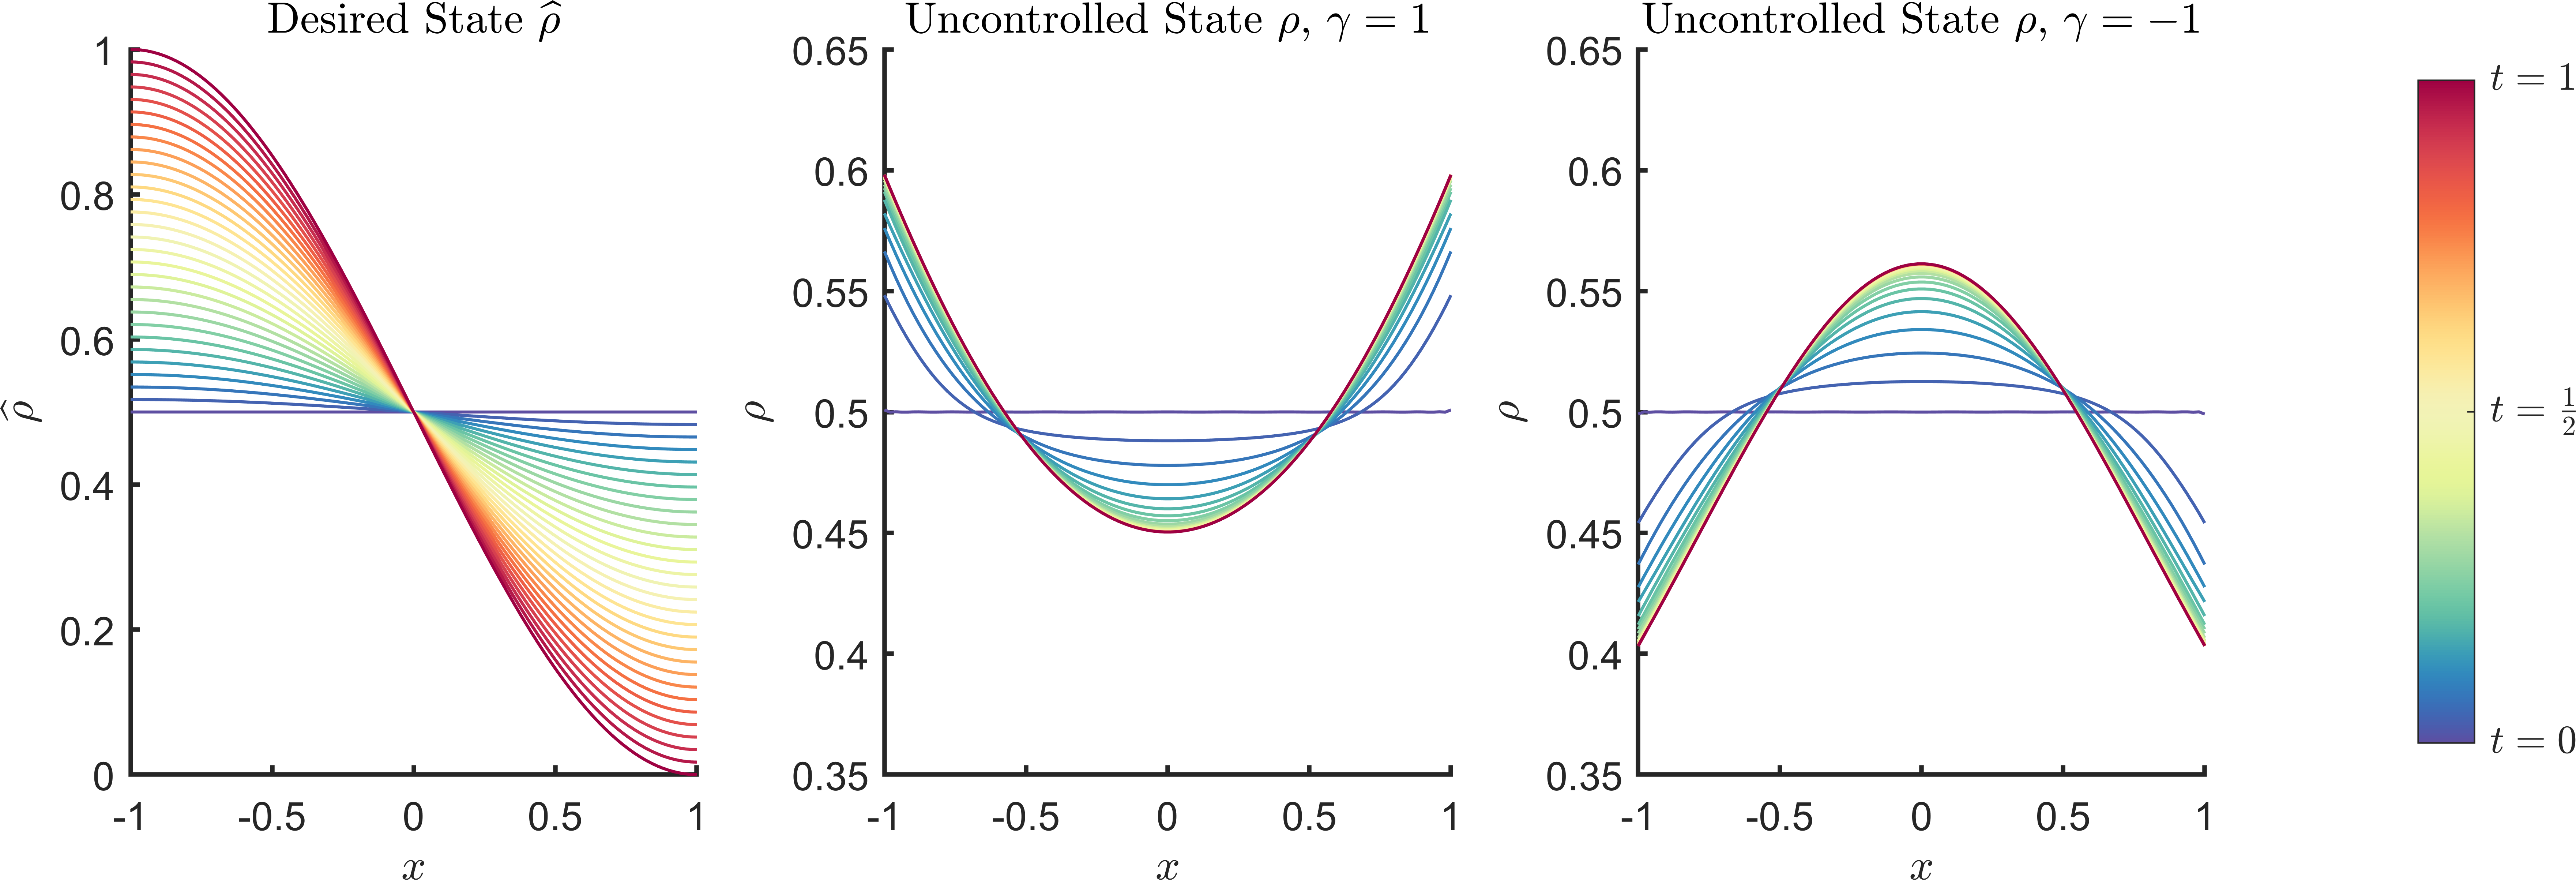
\includegraphics[scale=0.05]{Figure1.png}
	\caption{Example 1, desired state $\widehat \rho$ and uncontrolled state $\rho$ at $\gamma =1$ and $\gamma =-1$}
	\label{Ex12DN1}
\end{figure}
\begin{figure}[h]
	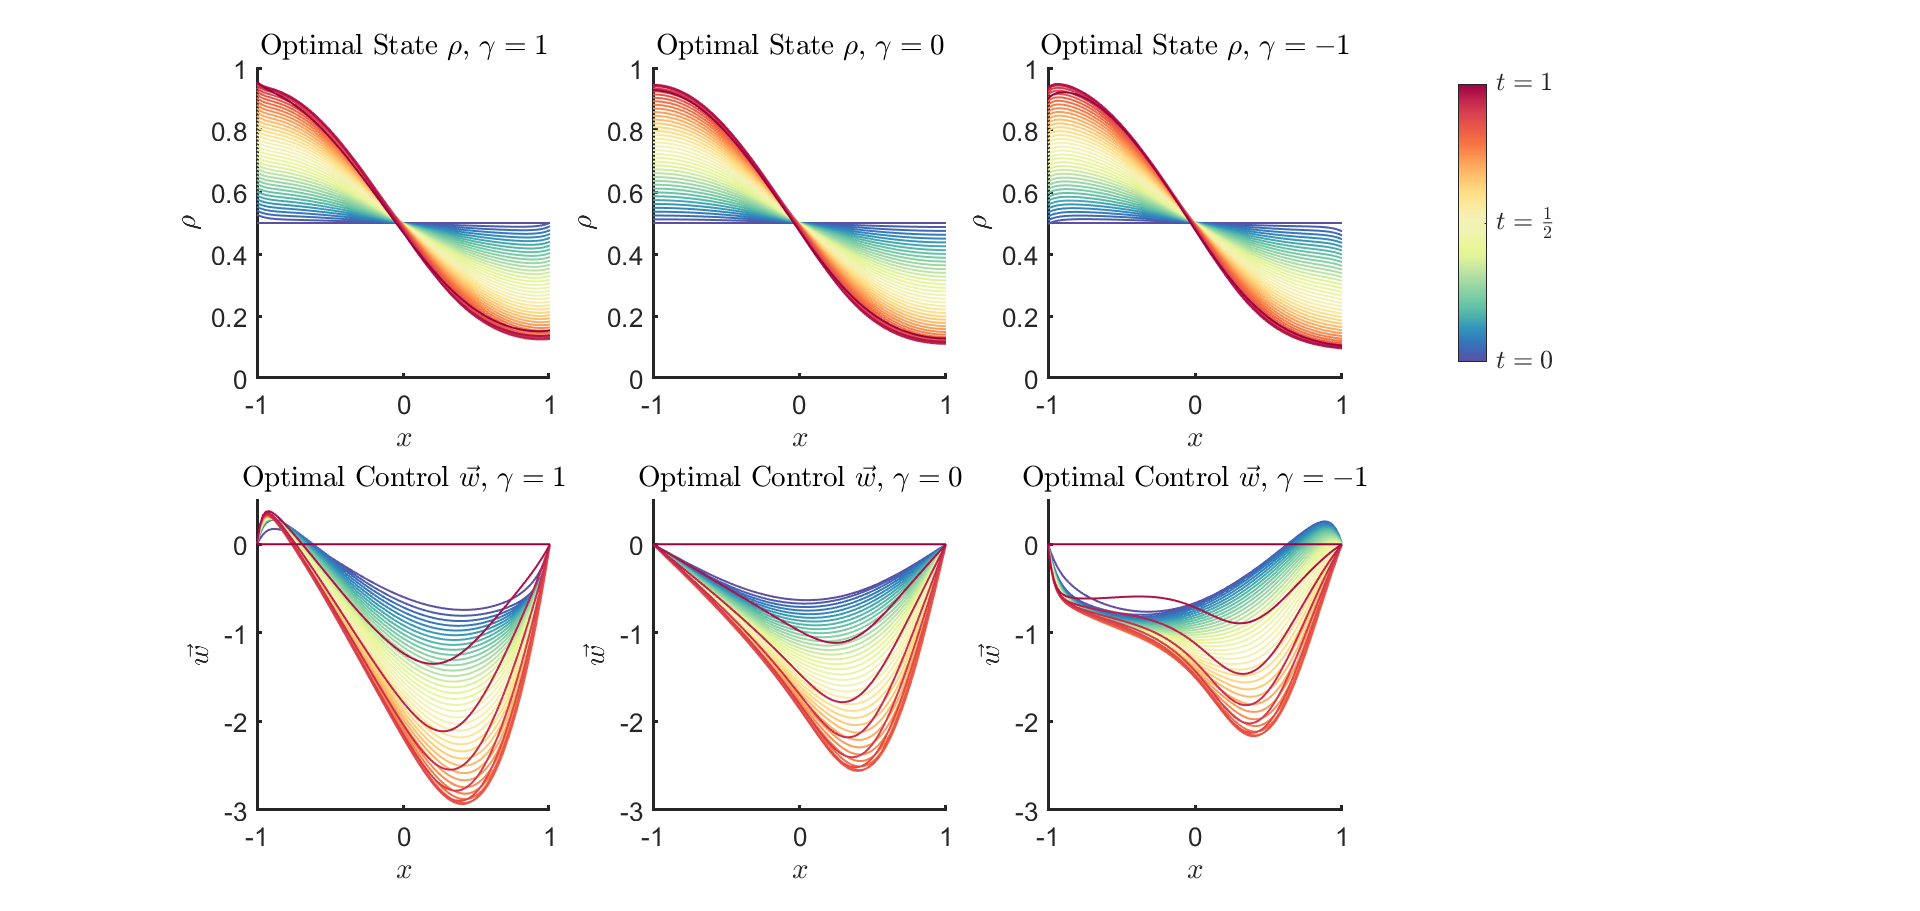
\includegraphics[scale=0.05]{Figure2.png}
	\caption{Example 1, optimal state $\rho$ and the corresponding optimal control $\vec{w}$ for $\gamma = 1,0,-1$, $\beta = 10^{-3}$.}
	\label{Ex12DN2}
\end{figure}

\begin{table}
\begin{tabular}{ | c | c || c | c | c | c ||}
\hline
\multicolumn{2}{|c||}{}& $\beta = 10^{-3}$ & $\beta = 10^{-1}$ & $\beta = 10^{1}$ & $\beta = 10^{3}$  \\
\hline
\hline
 & $\mathcal{J}_{uc}$ & $\numprint{0.0438}$ & $\numprint{0.0438}$ & $\numprint{0.0438}$ & $\numprint{0.0438}$ \\
$\kappa= \numprint{-1}$  & $\mathcal{J}_c$ & $\numprint{0.0011}$ & $\numprint{0.0267}$ & $\numprint{0.0435}$ & $\numprint{0.0438}$ \\
& \texttt{Iter} & $\numprint{670}$ & $\numprint{650}$ & $\numprint{449}$ & $\numprint{1}$ \\
\hline
 & $\mathcal{J}_{uc}$ & $\numprint{0.0417}$ & $\numprint{0.0417}$ & $\numprint{0.0417}$ & $\numprint{0.0417}$ \\
$\kappa= \numprint{0}$  & $\mathcal{J}_c$ & $\numprint{0.0014}$ & $\numprint{0.0283}$ & $\numprint{0.0415}$ & $\numprint{0.0417}$ \\
& \texttt{Iter} & $\numprint{665}$ & $\numprint{656}$ & $\numprint{434}$ & $\numprint{1}$ \\
\hline
 & $\mathcal{J}_{uc}$ & $\numprint{0.0434}$ & $\numprint{0.0434}$ & $\numprint{0.0434}$ & $\numprint{0.0434}$ \\
$\kappa= \numprint{1}$  & $\mathcal{J}_c$ & $\numprint{0.0020}$ & $\numprint{0.0322}$ & $\numprint{0.0432}$ & $\numprint{0.0434}$ \\
& \texttt{Iter} & $\numprint{654}$ & $\numprint{682}$ & $\numprint{422}$ & $\numprint{1}$ \\
\hline
\end{tabular}
\caption{Example 1: Uncontrolled cost $\mathcal{J}_{uc}$, optimal control cost $\mathcal{J}_{c}$, and number of iterations \emph{\texttt{Iter}}, for a range of $\kappa$ and $\beta$ values.}
\label{TabS5:Prob1}
\end{table} %\label{TabS5:Prob1}
%\begin{table}[h]
%	\begin{tabular}{ ||c|| c | c |c | c ||}
%		\hline
%		$\beta$ / $\gamma$ & $10^{-3}$  & $10^{-1}$  & $10$ & $10^3$ \\ 
%		\hline 
%		      & $J_{uc} = 0.0438$ & $J_{uc} = 0.0438$  & $J_{uc} = 0.0438$ & $J_{uc} = 0.0438$\\ 
%		 $-1$ & $J_c = 0.0011$ & $J_c = 0.0270$ & $J_c = 0.0435$ & $J_c = 0.0438$\\ 
%		      & Iter. $= 667$ & Iter. $= 649$  & Iter. $= 468$ & Iter. $= 13$\\ 
%		 \hline
%		      & $J_{uc} = 0.0417$ & $J_{uc} = 0.0417$   & $J_{uc} = 0.0417$& $J_{uc} = 0.0417$\\
%		 $0$  & $J_c = 0.0014$ & $J_c = 0.0283$  & $J_c = 0.0415$ & $J_c = 0.0417$\\ 
%		      & Iter. $= 671$ & Iter. $= 656$  & Iter. $= 434$ & Iter. $= 1$\\ 
%		 \hline
%		      & $J_{uc} = 0.0434$ & $J_{uc} = 0.0434$  & $J_{uc} = 0.0434$ & $J_{uc} = 0.0434$\\
%		 $1$  & $J_c = 0.0020$ & $J_c = 0.0324$  & $J_c = 0.0432$ & $J_c = 0.0434$\\ 
%		      & Iter. $= 674$ & Iter. $= 686$  & Iter. $= 411$ & Iter. $= 1$\\ 
%		 \hline 
%	\end{tabular}
%    \caption{}
%    \label{TabNFlowEx1}
%\end{table}

\subsubsection{Neumann boundary conditions, Example 2} 
The chosen inputs for Example 2 are:
\begin{align*}
&\widehat \rho = \bigg(\frac{1}{2}\cos(\pi y) + \frac{1}{2}\bigg)(1-t) + t\bigg(-\frac{1}{2}\cos(2 \pi y) + \frac{1}{2}\bigg),\\
&\rho_{0} = \frac{1}{2}\cos(\pi y) + \frac{1}{2},\ \
\adj_{T} = 0,\ \
\vec{w} = \vec{0},\ \
f =0,\ \
V_{ext} =0.
\end{align*}
In Table \ref{TabS5:Prob2} the results for Example 2 are displayed. These are comparable with the results for Example 1, in the effect of $\beta$ and the number of iterations. In all three configurations of the interaction term, the control is focussed on transporting the mass from the middle of the domain onto two piles centred at $x=-0.5$ and $x=0.5$. In Figure \ref{Ex22DN1}, the desired state $\widehat \rho$, the optimal state $\rho$ and the optimal control $\vec{w}$ are displayed for $\beta = 10^{-3}$ and $\gamma = 1$, and compared to Example 3 below. 
\begin{figure}[h]
	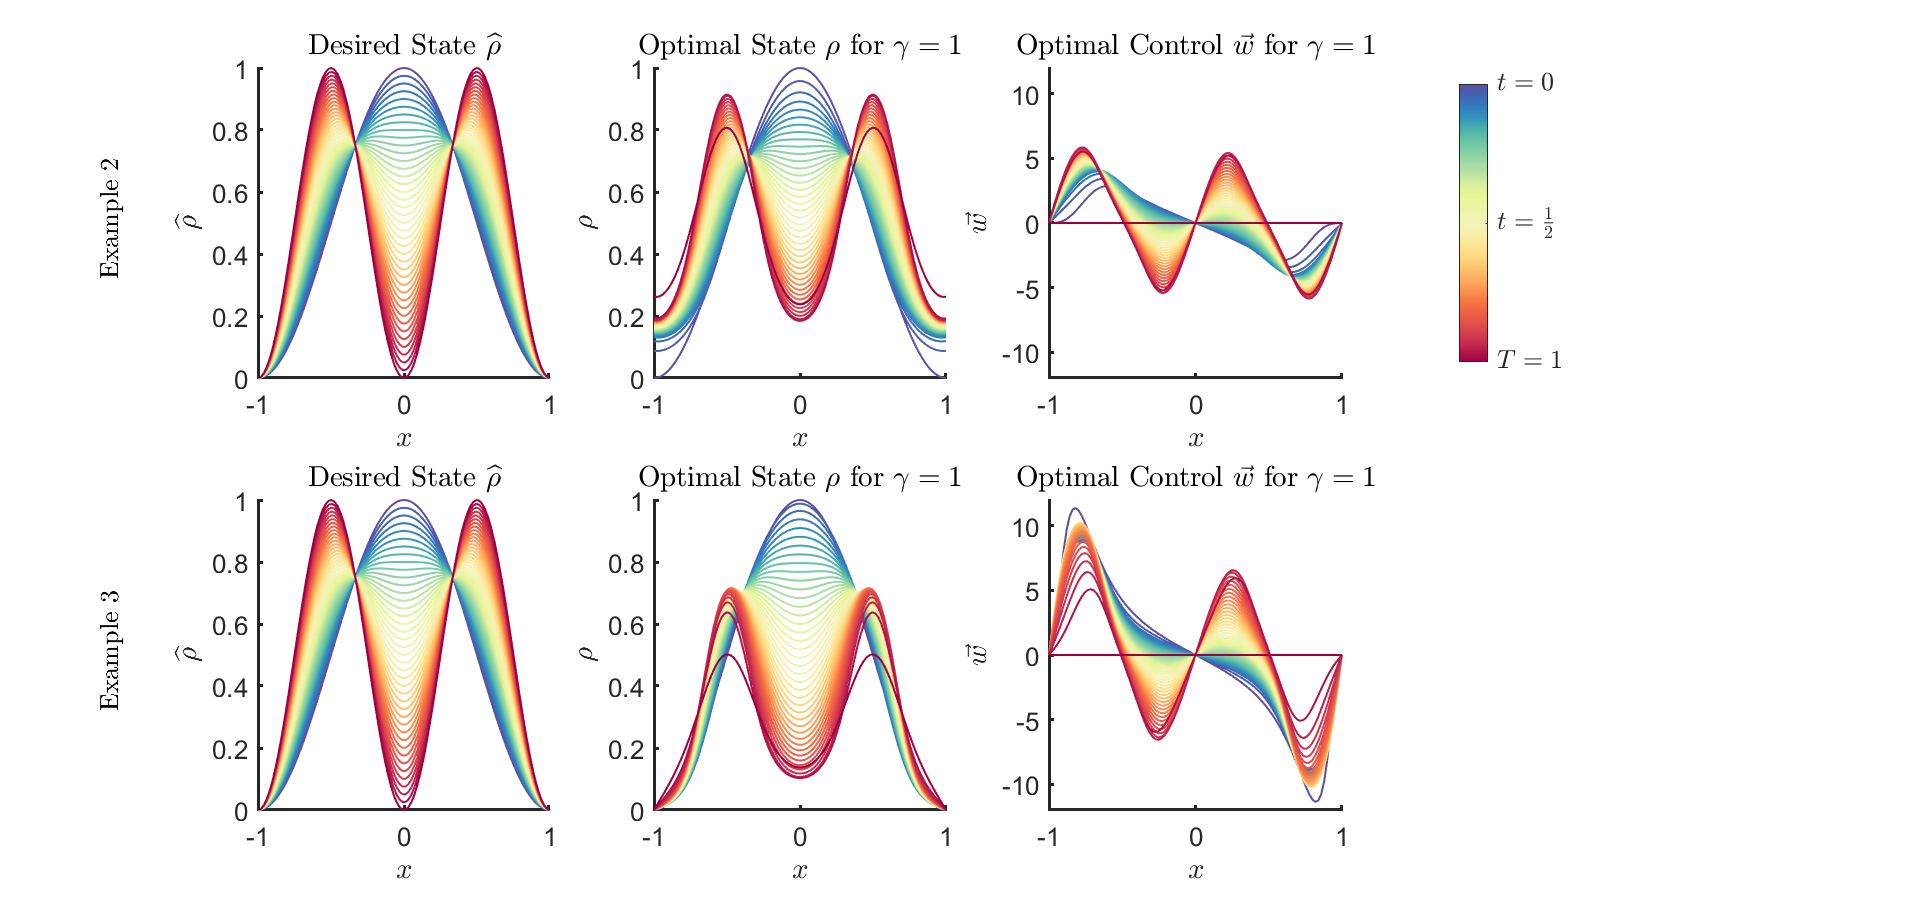
\includegraphics[scale=0.05]{Figure3.png}
	\caption{Example 2/ Example 3, desired state $\widehat \rho$, optimal state $\rho$ and corresponding optimal control $\vec{w}$, $\beta = 10^{-3}$, $\gamma = 1$.}
	\label{Ex22DN1}
\end{figure}

\begin{table}
\begin{tabular}{ | c | c || c | c | c | c ||}
\hline
\multicolumn{2}{|c||}{}& $\beta = 10^{-3}$ & $\beta = 10^{-1}$ & $\beta = 10^{1}$ & $\beta = 10^{3}$  \\
\hline
\hline
 & $\mathcal{J}_{uc}$ & $\numprint{0.0536}$ & $\numprint{0.0536}$ & $\numprint{0.0536}$ & $\numprint{0.0536}$ \\
$\kappa= \numprint{-1}$  & $\mathcal{J}_c$ & $\numprint{0.0096}$ & $\numprint{0.0492}$ & $\numprint{0.0535}$ & $\numprint{0.0536}$ \\
& \texttt{Iter} & $\numprint{715}$ & $\numprint{767}$ & $\numprint{367}$ & $\numprint{1}$ \\
\hline
 & $\mathcal{J}_{uc}$ & $\numprint{0.0669}$ & $\numprint{0.0669}$ & $\numprint{0.0669}$ & $\numprint{0.0669}$ \\
$\kappa= \numprint{0}$  & $\mathcal{J}_c$ & $\numprint{0.0109}$ & $\numprint{0.0603}$ & $\numprint{0.0668}$ & $\numprint{0.0669}$ \\
& \texttt{Iter} & $\numprint{714}$ & $\numprint{770}$ & $\numprint{390}$ & $\numprint{1}$ \\
\hline
 & $\mathcal{J}_{uc}$ & $\numprint{0.0839}$ & $\numprint{0.0839}$ & $\numprint{0.0839}$ & $\numprint{0.0839}$ \\
$\kappa= \numprint{1}$  & $\mathcal{J}_c$ & $\numprint{0.0125}$ & $\numprint{0.0748}$ & $\numprint{0.0838}$ & $\numprint{0.0839}$ \\
& \texttt{Iter} & $\numprint{713}$ & $\numprint{773}$ & $\numprint{403}$ & $\numprint{1}$ \\
\hline
\end{tabular}
\caption{Example 2: Cost when $\vec{w}=\vec{0}$, optimal control cost, and iterations required, for a range of $\kappa$, $\beta$.}
\label{TabS5:Prob2}
\end{table} %\label{TabS5:Prob2a}
%
%\begin{table}
%	\begin{tabular}{ ||c|| c | c |c | c ||}
%		\hline
%		$\beta$ / $\gamma$ & $10^{-3}$  & $10^{-1}$  & $10$ & $10^3$ \\ 
%		\hline 
%		& $J_{uc} = 0.0536$ & $J_{uc} = 0.0536$  & $J_{uc} = 0.0536$ & $J_{uc} = 0.0536$\\ 
%		$-1$ & $J_c = 0.0096$ & $J_c = 0.0493$ & $J_c = 0.0535$ & $J_c = 0.0536$\\ 
%		& Iter. $= 724$ & Iter. $= 769$  & Iter. $= 379$ & Iter. $= 1$\\ 
%		\hline
%		& $J_{uc} = 0.0669$ & $J_{uc} = 0.0669$   & $J_{uc} = 0.0669$& $J_{uc} = 0.0669$\\
%		$0$  & $J_c = 0.0109$ & $J_c = 0.0603$  & $J_c = 0.0668$ & $J_c = 0.0669$\\ 
%		& Iter. $= 726$ & Iter. $= 770$  & Iter. $= 390$ & Iter. $= 1$\\ 
%		\hline
%		& $J_{uc} = 0.0839$ & $J_{uc} = 0.0839$  & $J_{uc} = 0.0839$ & $J_{uc} = 0.0839$\\
%		$1$  & $J_c = 0.0125$ & $J_c = 0.0749$  & $J_c = 0.0838$ & $J_c = 0.0839$\\ 
%		& Iter. $= 728$ & Iter. $= 772$  & Iter. $= 396$ & Iter. $= 1$\\ 
%		\hline 
%	\end{tabular}
%    \caption{}
%    \label{TabNFlowEx2}
%\end{table}

\subsubsection{Dirichlet boundary conditions, Example 3} 
The inputs for this example are:
\begin{align*}
&\widehat \rho = \bigg(\frac{1}{2}\cos(\pi y) + \frac{1}{2}\bigg)(1-t) + t\bigg(-\frac{1}{2}\cos(2 \pi y) + \frac{1}{2}\bigg),\\
&\rho_{0} = \frac{1}{2}\cos(\pi y) + \frac{1}{2},\ \
\adj_{T} = 0,\ \
\vec{w} = \vec{0},\ \
f =0,\ \
V_{ext} =0.
\end{align*}
Table \ref{TabS5:Prob3} presents the results for this example, for a range of $\beta$ values and different interaction strengths. The observations are in line with those in Example 1 and 2. In particular, $ \widehat \rho$ and $\rho_0$ coincide with those of the problem with Neumann boundary conditions in Example 2. A comparison between the two examples is illustrated in Figure \ref{Ex22DN1}. Both the optimal state $\rho$ and the optimal control are qualitatively different when considering Dirichlet boundary conditions over Neumann conditions. The numerical result for this example was achieved with $N=40$ and $n = 30$, rather than with $N=30$ and $n=20$. This indicates that the Dirichlet boundary conditions are harder to apply in this problem, due to the steep shape of the desired state. This steepness is somewhat less impactful in Example 2, where the desired state is not closely matched by the optimal state at the boundaries. In Example 3, while the optimal state matches the desired state perfectly at the boundary, the peaks of the desired state are matched less closely. In Figure \ref{Ex22DN1}, this can be confirmed by considering the control plots. The optimal control for Example 3 is larger than for Example 2, specifically between the boundaries of the domain and the peaks of the desired state, indicating difficulties in this region.
\begin{table}
\begin{tabular}{ ||c|| c | c | c | c | c ||}
\hline
& & $\beta = 10^{-3}$ & $\beta = 10^{-1}$ & $\beta = 10^{1}$ & $\beta = 10^{3}$  \\
\hline
 & $J_{uc}$ & $\numprint{1.4165e-1}$ & $\numprint{1.4165e-1}$ & $\numprint{1.4165e-1}$ & $\numprint{1.4165e-1}$ \\
$\gamma= \numprint{-1}$  & $J_c$ & $\numprint{3.5594e-2}$ & $\numprint{1.3270e-1}$ & $\numprint{1.4155e-1}$ & $\numprint{1.4165e-1}$ \\
& $Iter.$ & $\numprint{944}$ & $\numprint{816}$ & $\numprint{437}$ & $\numprint{1}$ \\
\hline
 & $J_{uc}$ & $\numprint{1.5452e-1}$ & $\numprint{1.5452e-1}$ & $\numprint{1.5452e-1}$ & $\numprint{1.5452e-1}$ \\
$\gamma= \numprint{0}$  & $J_c$ & $\numprint{3.8023e-2}$ & $\numprint{1.4549e-1}$ & $\numprint{1.5442e-1}$ & $\numprint{1.5452e-1}$ \\
& $Iter.$ & $\numprint{940}$ & $\numprint{825}$ & $\numprint{440}$ & $\numprint{1}$ \\
\hline
 & $J_{uc}$ & $\numprint{1.6610e-1}$ & $\numprint{1.6610e-1}$ & $\numprint{1.6610e-1}$ & $\numprint{1.6610e-1}$ \\
$\gamma= \numprint{1}$  & $J_c$ & $\numprint{4.1143e-2}$ & $\numprint{1.5751e-1}$ & $\numprint{1.6601e-1}$ & $\numprint{1.6610e-1}$ \\
& $Iter.$ & $\numprint{932}$ & $\numprint{827}$ & $\numprint{440}$ & $\numprint{1}$ \\
\hline
\end{tabular}
\caption{Problem 3 ($n = 30,N = 40$)}
\label{TabS5:Prob3}
\end{table} %\label{TabS5:Prob3}
%\begin{table}
%	\begin{tabular}{ ||c|| c | c |c | c ||}
%		\hline
%		$\beta$ / $\gamma$ & $10^{-3}$  & $10^{-1}$  & $10$ & $10^3$ \\ 
%		\hline 
%		& $J_{uc} = 0.0510$ & $J_{uc} = 0.0510$  & $J_{uc} = 0.0510$ & $J_{uc} = 0.0510$\\ 
%		$-1$ & $J_c = 0.0026$ & $J_c = 0.0365$ & $J_c = 0.0508$ & $J_c = 0.0510$\\ 
%		& Iter. $= 690$ & Iter. $= 696$  & Iter. $= 696$ & Iter. $= 696$\\ 
%		\hline
%		& $J_{uc} = 0.0417$ & $J_{uc} = 0.0417$  & $J_{uc} = 0.0417$& $J_{uc} = 0.0417$\\
%		$0$  & $J_c = 0.0027$ & $J_c = 0.0343$  & $J_c = 0.0416$ & $J_c = 0.0417$\\ 
%		& Iter. $= 696$ & Iter. $= 742$  & Iter. $= 409$ & Iter. $= 1$\\ 
%		\hline
%		& $J_{uc} = 0.0452$ & $J_{uc} = 0.0452$  & $J_{uc} = 0.0452$ & $J_{uc} = 0.0452$\\
%		$1$  & $J_c = 0.0030$ & $J_c = 0.0388$  & $J_c = 0.0452$ & $J_c = 0.0452$\\ 
%		& Iter. $= 703$ & Iter. $= 779$  & Iter. $= 397$ & Iter. $= 1$\\ 
%		\hline 
%	\end{tabular}
%	\caption{Update table! Is for different example}
%	\label{TabNFlowEx3}
%\end{table}


\subsection{Linear control problems with an additional nonlocal integral term}
In this section, examples of solving Problem \eqref{AdvDiff_Linear} with both 'no-flux type' boundary conditions \eqref{NoFlux_Linear} and Dirichlet boundary conditions \eqref{Dirichlet}.
\subsubsection{Dirichlet boundary conditions, Example 4}
The inputs for this example are:
\begin{align*}
&\widehat \rho = (1 - t)\bigg(\frac{1}{2}\cos(\pi y) + \frac{1}{2}\bigg)  + t\bigg(-\frac{1}{2}\cos(\pi y) + \frac{1}{2}\bigg),\\
&\rho_{0} = \frac{1}{2}\cos(\pi y) + \frac{1}{2},\ \
\adj_{T} = 0,\ \
{w} = 0,\ \
f =0, \ \
V_{ext} =0.
\end{align*}
In Table \ref{TabS5:Prob4} the results for Example 4 for a range of parameter values can be found. The results are qualitatively similar to the previous examples, the only difference is that the control is applied linearly in this example. (++also same $\widehat \rho$ and $\rho_0$ as Example 2 and 3. May want to change this++)
\begin{table}
\begin{tabular}{ | c | c || c | c | c | c ||}
\hline
\multicolumn{2}{|c||}{}& $\beta = 10^{-3}$ & $\beta = 10^{-1}$ & $\beta = 10^{1}$ & $\beta = 10^{3}$  \\
\hline
\hline
 & $\mathcal{J}_{uc}$ & $\numprint{0.1394}$ & $\numprint{0.1394}$ & $\numprint{0.1394}$ & $\numprint{0.1394}$ \\
$\kappa= \numprint{-1}$  & $\mathcal{J}_c$ & $\numprint{0.0183}$ & $\numprint{0.0862}$ & $\numprint{0.1384}$ & $\numprint{0.1394}$ \\
& \texttt{Iter} & $\numprint{1575}$ & $\numprint{1486}$ & $\numprint{1026}$ & $\numprint{117}$ \\
\hline
 & $\mathcal{J}_{uc}$ & $\numprint{0.1526}$ & $\numprint{0.1526}$ & $\numprint{0.1526}$ & $\numprint{0.1526}$ \\
$\kappa= \numprint{0}$  & $\mathcal{J}_c$ & $\numprint{0.0183}$ & $\numprint{0.0983}$ & $\numprint{0.1516}$ & $\numprint{0.1526}$ \\
& \texttt{Iter} & $\numprint{1582}$ & $\numprint{1474}$ & $\numprint{1023}$ & $\numprint{113}$ \\
\hline
 & $\mathcal{J}_{uc}$ & $\numprint{0.1645}$ & $\numprint{0.1645}$ & $\numprint{0.1645}$ & $\numprint{0.1645}$ \\
$\kappa= \numprint{1}$  & $\mathcal{J}_c$ & $\numprint{0.0189}$ & $\numprint{0.1103}$ & $\numprint{0.1635}$ & $\numprint{0.1645}$ \\
& \texttt{Iter} & $\numprint{1589}$ & $\numprint{1465}$ & $\numprint{1022}$ & $\numprint{112}$ \\
\hline
\end{tabular}
\caption{Example 4: Uncontrolled cost $\mathcal{J}_{uc}$, optimal cost $\mathcal{J}_{c}$, and number of iterations, for a range of $\kappa$ and $\beta$ values.}
\label{TabS5:Prob4}
\end{table} %\label{TabS5:Prob4}

%\begin{table}[h]
%	\begin{tabular}{ ||c|| c | c |c | c ||}
%		\hline
%		$\beta$ / $\gamma$ & $10^{-3}$  & $10^{-1}$  & $10$ & $10^3$ \\ 
%		\hline 
%		& $J_{uc} = 0.1417$ & $J_{uc} = 0.1417$  & $J_{uc} = 0.1417$ & $J_{uc} = 0.1417$\\ 
%		$-1$ & $J_c = 0.0203$ & $J_c = 0.0903$ & $J_c = 0.1407$ & $J_c = 0.1417$\\ 
%		& Iter. $= 787$ & Iter. $= 740$  & Iter. $= 503$ & Iter. $= 49$\\ 
%		\hline
%		& $J_{uc} = 0.1545$ & $J_{uc} = 0.1545$   & $J_{uc} = 0.1545$& $J_{uc} = 0.1545$\\
%		$0$  & $J_c = 0.0200$ & $J_c = 0.1015$  & $J_c = 0.1536$ & $J_c = 0.1545$\\ 
%		& Iter. $= 791$ & Iter. $= 740$  & Iter. $= 510$ & Iter. $= 56$\\ 
%		\hline
%		& $J_{uc} = 0.1661$ & $J_{uc} = 0.1661$  & $J_{uc} = 0.1661$ & $J_{uc} = 0.1661$\\
%		$1$  & $J_c = 0.0204$ & $J_c = 0.1135$  & $J_c = 0.1652$ & $J_c = 0.1661$\\ 
%		& Iter. $= 795$ & Iter. $= 741$  & Iter. $= 515$ & Iter. $= 61$\\ 
%		\hline 
%	\end{tabular}
%	\caption{}
%	\label{TabNFlowEx4}
%\end{table}


\subsubsection{Neumann boundary conditions, Example 5}
The inputs for this example are:
\begin{align*}
&\widehat \rho = \frac{1}{2}(1-t) + t\frac{1}{2}(-\cos(\pi y) + 1),\\
&\rho_{0} = \frac{1}{2},\ \
\adj_{T} = 0,\ \
{w} = 0,\ \
f =0,\ \
V_{ext} =0.
\end{align*}
Table \ref{TabS5:Prob5} shows the results for Example 5. Note that for this example, when $\beta = 10^{-3}$, the mixing parameter $\lambda$ had to be set to $0.001$, to guarantee stable convergence of the method (why? explanation needed?).
Again, the only qualitative difference to interpreting the results is that the control is applied linearly.
\begin{table}
\begin{tabular}{ ||c|| c | c | c | c | c ||}
\hline
& & $\beta = 10^{-3}$ & $\beta = 10^{-1}$ & $\beta = 10^{1}$ & $\beta = 10^{3}$  \\
\hline
 & $J_{uc}$ & $\numprint{6.0640e-2}$ & $\numprint{6.0640e-2}$ & $\numprint{6.0640e-2}$ & $\numprint{6.0640e-2}$ \\
$\gamma= \numprint{-1}$  & $J_c$ & $\numprint{6.0180e-3}$ & $\numprint{5.5365e-2}$ & $\numprint{6.0592e-2}$ & $\numprint{6.0640e-2}$ \\
& $Iter.$ & $\numprint{7320}$ & $\numprint{7712}$ & $\numprint{3888}$ & $\numprint{1}$ \\
\hline
 & $J_{uc}$ & $\numprint{4.1667e-2}$ & $\numprint{4.1667e-2}$ & $\numprint{4.1667e-2}$ & $\numprint{4.1667e-2}$ \\
$\gamma= \numprint{0}$  & $J_c$ & $\numprint{4.5414e-3}$ & $\numprint{3.8334e-2}$ & $\numprint{4.1632e-2}$ & $\numprint{4.1667e-2}$ \\
& $Iter.$ & $\numprint{7271}$ & $\numprint{7614}$ & $\numprint{3643}$ & $\numprint{1}$ \\
\hline
 & $J_{uc}$ & $\numprint{2.8551e-2}$ & $\numprint{2.8551e-2}$ & $\numprint{2.8551e-2}$ & $\numprint{2.8551e-2}$ \\
$\gamma= \numprint{1}$  & $J_c$ & $\numprint{3.5942e-3}$ & $\numprint{2.6480e-2}$ & $\numprint{2.8529e-2}$ & $\numprint{2.8551e-2}$ \\
& $Iter.$ & $\numprint{7249}$ & $\numprint{7482}$ & $\numprint{3410}$ & $\numprint{1}$ \\
\hline
\end{tabular}
\caption{Problem 5}
\label{TabS5:Prob5}
\end{table} %\label{TabS5:Prob5}
%\begin{table}[h]
%	\begin{tabular}{ ||c|| c | c |c | c ||}
%		\hline
%		$\beta$ / $\gamma$ & $10^{-3}$  & $10^{-1}$  & $10$ & $10^3$ \\ 
%		\hline 
%		& $J_{uc} = 0.0606$ & $J_{uc} = 0.0606$  & $J_{uc} = 0.0606$ & $J_{uc} = 0.0606$\\ 
%		$-1$ & $J_c = 0.0060$ & $J_c = 0.0554$ & $J_c = 0.0606$ & $J_c = 0.0606$\\ 
%		& Iter. $= 7311$ & Iter. $= 771$  & Iter. $= 389$ & Iter. $= 1$\\ 
%		\hline
%		& $J_{uc} = 0.0417$ & $J_{uc} = 0.0417$   & $J_{uc} = 0.0417$& $J_{uc} = 0.0417$\\
%		$0$  & $J_c = 0.0045$ & $J_c = 0.0383$  & $J_c = 0.0416$ & $J_c = 0.0417$\\ 
%		& Iter. $= 7227$ & Iter. $= 759$  & Iter. $= 364$ & Iter. $= 1$\\ 
%		\hline
%		& $J_{uc} = 0.0286$ & $J_{uc} = 0.0286$  & $J_{uc} = 0.0286$ & $J_{uc} = 0.0286$\\
%		$1$  & $J_c = 0.0036$ & $J_c = 0.0265$  & $J_c = 0.0285$ & $J_c = 0.0286$\\ 
%		& Iter. $= 7205$ & Iter. $= 746$  & Iter. $= 341$ & Iter. $= 1$\\ 
%		\hline 
%	\end{tabular}
%	\caption{}
%	\label{TabNFlowEx5}
%\end{table}


\subsection{Nonlinear control problems with an additional nonlocal integral term in 2D}
In this section, two-dimensional examples are considered, to illustrate the fact that the application of the method differs very little from the one dimensional setting. The main difference is that in nonlinear control problems the control is a two-dimensional vector field. Furthermore, the number of spatial points increases from $N$ to $N_1\times N_2$, which makes computations much more costly. Compensating for this increased cost is one of the motivations to develop fast optimization solvers, such as the fixed point method introduced in Section \ref{sec:Method_Solver}.
\subsubsection{Neumann boundary conditions, Example 1}	
We have the following set up:
\begin{align*}
&\widehat \rho = \frac{1}{4}(1-t) + t\bigg(\frac{1}{4}\sin \bigg(\frac{\pi}{2}(x_1 - 2)\bigg)\sin \bigg(\frac{\pi}{2}(x_2 - 2)\bigg) + \frac{1}{4}\bigg),\\
&\rho_0 = \frac{1}{4},\ \
q_{T} = 0,\ \
\vec{w} = \vec{0},\ \
f =0,\ \
V_{ext} =0.
\end{align*}
This example is the two dimensional version of Example 1 in Section \ref{sec:Examples1d}. The results for this example are displayed in Table \ref{TabS5:Prob12D}. In Figures \ref{rhoHat2dEx2} it can be observed that as in Example 1 in Section \ref{sec:Examples1d}, the uncontrolled state forms a cluster in the centre of the domain, due to the attractive interactions. Figure \ref{rhoOpt2dEx2} shows the optimal state and control for different time points, for $\beta = 10^{-3}$ and $\gamma = -1$. Here, the control through a vector field illustrates why nonlinear control is called 'flow control'. 

\begin{table}
\begin{tabular}{ ||c|| c | c | c | c | c ||}
\hline
& & $\beta = 10^{-3}$ & $\beta = 10^{-1}$ & $\beta = 10^{1}$ & $\beta = 10^{3}$  \\
\hline
 & $\mathcal J_{\vec w = \vec 0}$ & $0.0113$ & $0.0113$ & $0.0113$ & $0.0113$ \\
$\kappa= -1$  & $\mathcal J_{Opt}$ & $0.0013$ & $0.0104$ & $0.0113$ & $0.0113$ \\
& $\text{Iterations}$ & $676$ & $700$ & $290$ & $1$ \\
\hline
\end{tabular}
\caption{Results for the test problem, with different $\beta$}
\label{TabS5:Prob12D}
\end{table} % \label{TabS5:Prob12D}

\begin{figure}[h]
	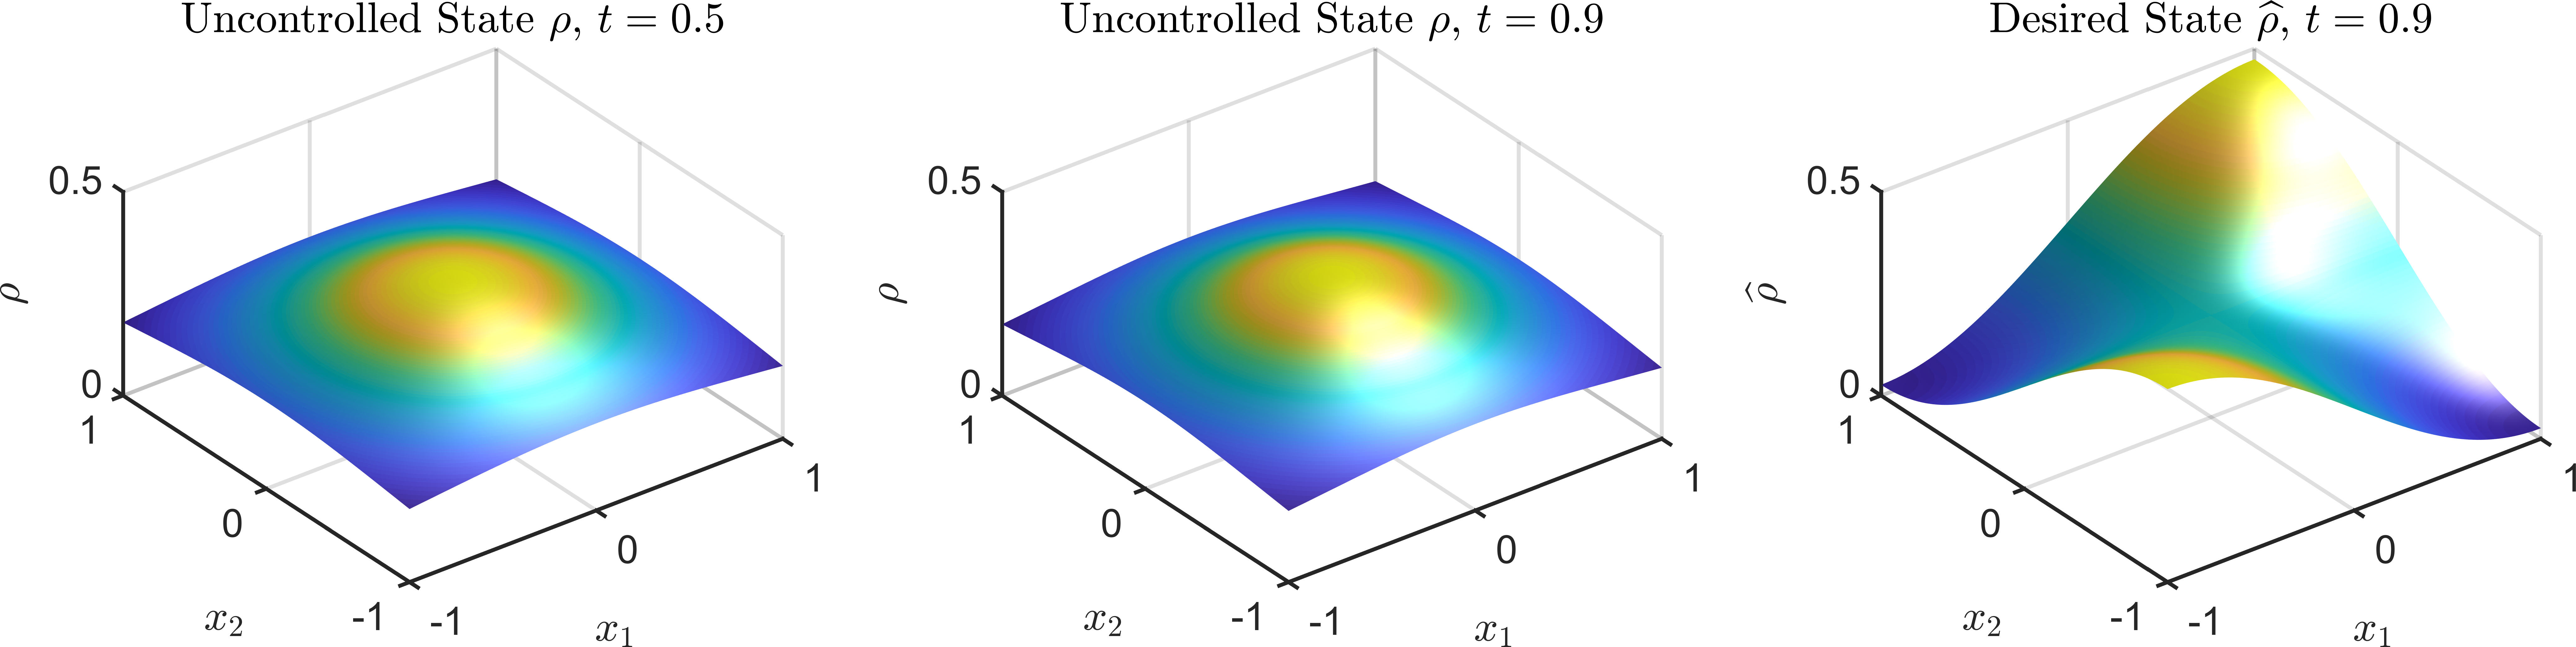
\includegraphics[scale=0.044]{Figure12D.png}
	\caption{2D Example 1, uncontrolled $\rho$ and $\widehat \rho$, $\beta = 10^{-3}$, $\gamma = -1$.}
	\label{rhoHat2dEx2}
\end{figure}
\begin{figure}[h]
	\includegraphics[scale=0.04]{Figure22D.png}
	\caption{2D Example 1, controlled $\rho$ and optimal control $\vec{w}$, $\beta = 10^{-3}$, $\gamma = -1$.}
	\label{rhoOpt2dEx2}
\end{figure}


\subsubsection{Neumann boundary conditions, Example 2}	
Here, we have:
\begin{align*}
&\widehat \rho = \frac{1}{4}(1-t) + t\frac{1}{0.9921}e^{-3((y_1+0.2)^2 + (y_2+0.2)^2))},\\
&\rho_0 = \frac{1}{4},\ \
q_{T} = 0,\ \
\vec{w} = \vec{0},\ \
f =0,\ \
V_{ext} =0.
\end{align*}
The numerical results for this example are displayed in Table \ref{TabS5:Prob22D}. In figures \ref{rhoHat2dEx4} and \ref{rhoOpt2dEx4} the results are illustrated for $\beta = 10^{-3}$ and $\gamma = -1$. It can be observed very clearly that the control is driving the particle distribution to the desired state. It is noticeable that the peak of the desired state does not have to be as supported as the slopes. This is due to the attractive interactions of the particles in this configuration, supporting the clustering at the peak, and cannot be observed for repulsive particles.


\begin{table}
\begin{tabular}{ | c | c || c | c | c | c ||}
\hline
\multicolumn{2}{|c||}{}& $\beta = 10^{-3}$ & $\beta = 10^{-1}$ & $\beta = 10^{1}$ & $\beta = 10^{3}$  \\
\hline
\hline
 & $\mathcal{J}_{uc}$ & $\numprint{0.0378}$ & $\numprint{0.0378}$ & $\numprint{0.0378}$ & $\numprint{0.0378}$ \\
$\kappa= \numprint{-1}$  & $\mathcal{J}_c$ & $\numprint{0.0017}$ & $\numprint{0.0312}$ & $\numprint{0.0377}$ & $\numprint{0.0378}$ \\
& \texttt{Iter} & $\numprint{691}$ & $\numprint{736}$ & $\numprint{347}$ & $\numprint{1}$ \\
\hline
 & $\mathcal{J}_{uc}$ & $\numprint{0.0478}$ & $\numprint{0.0478}$ & $\numprint{0.0478}$ & $\numprint{0.0478}$ \\
$\kappa= \numprint{0}$  & $\mathcal{J}_c$ & $\numprint{0.0064}$ & $\numprint{0.0450}$ & $\numprint{0.0478}$ & $\numprint{0.0478}$ \\
& \texttt{Iter} & $\numprint{718}$ & $\numprint{784}$ & $\numprint{343}$ & $\numprint{1}$ \\
\hline
 & $\mathcal{J}_{uc}$ & $\numprint{0.0526}$ & $\numprint{0.0526}$ & $\numprint{0.0526}$ & $\numprint{0.0526}$ \\
$\kappa= \numprint{1}$  & $\mathcal{J}_c$ & $\numprint{0.0137}$ & $\numprint{0.0514}$ & $\numprint{0.0526}$ & $\numprint{0.0526}$ \\
& \texttt{Iter} & $\numprint{735}$ & $\numprint{790}$ & $\numprint{338}$ & $\numprint{1}$ \\
\hline
\end{tabular}
\caption{2D Ex. 2: Uncontrolled cost $\mathcal{J}_{uc}$, optimal cost $\mathcal{J}_{c}$, and number of iterations, for a range of $\kappa$ and $\beta$ values.}
\label{TabS5:Prob22D}
\end{table} %\label{TabS5:Prob22D}

\begin{figure}[h]
	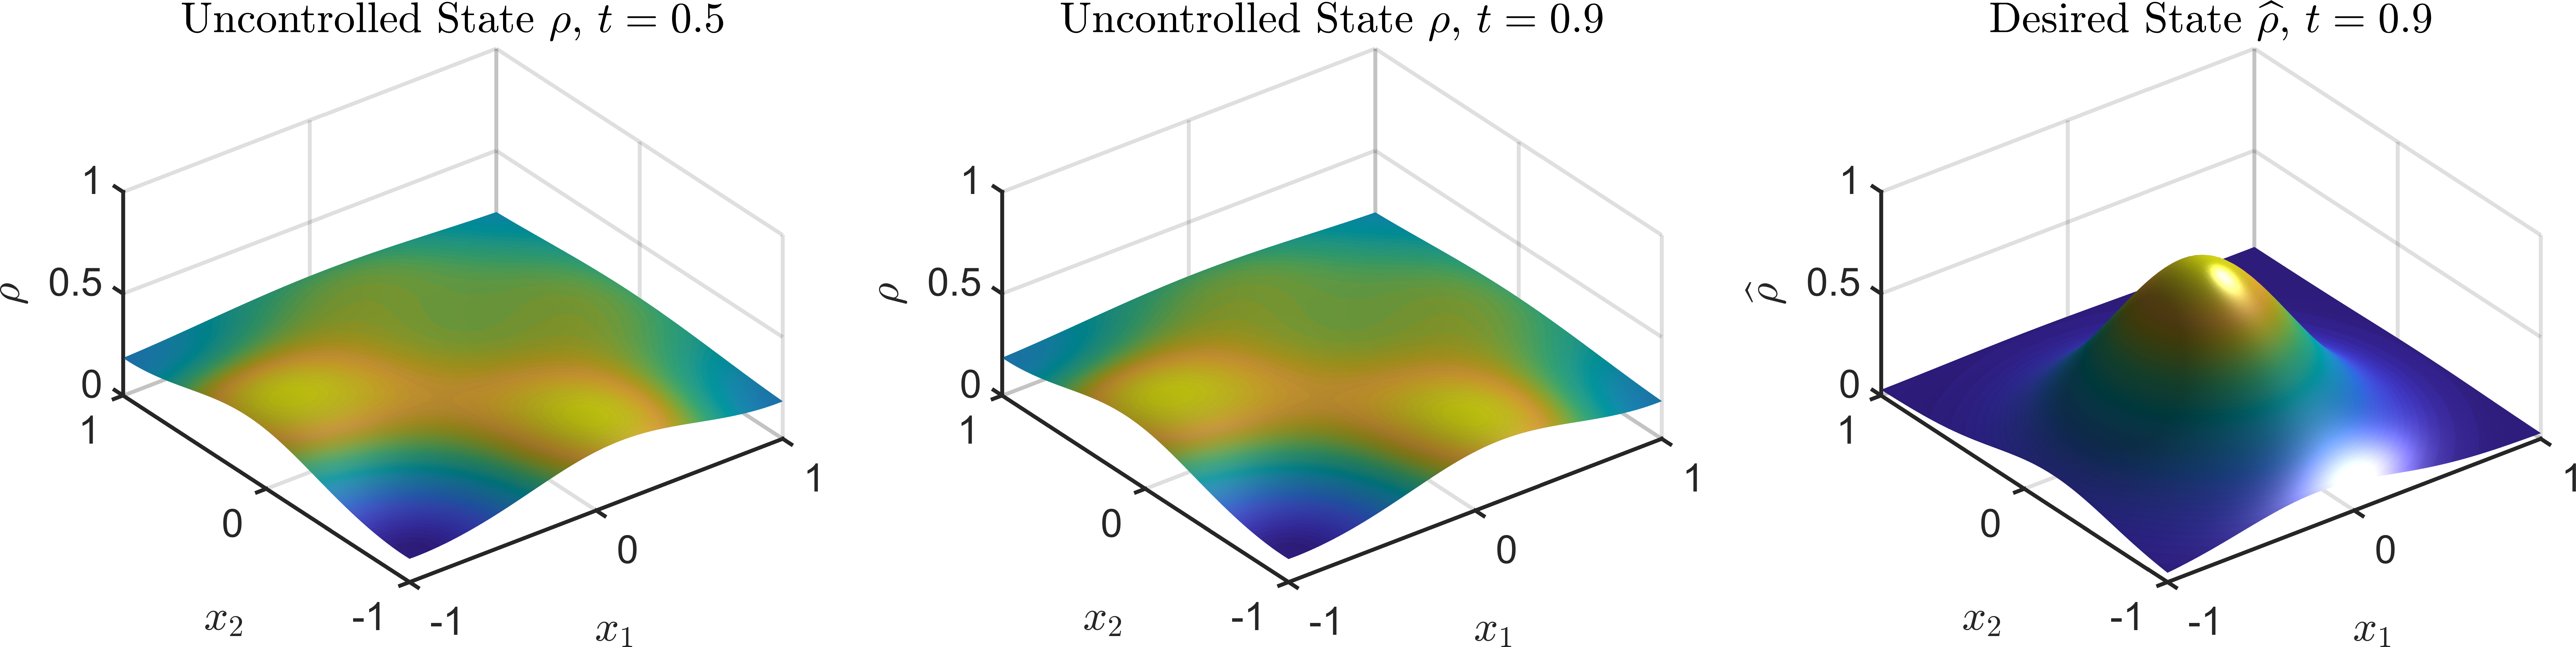
\includegraphics[scale=0.044]{Figure32D.png}
	\caption{2D Example 2, uncontrolled $\rho$ and $\widehat \rho$, $\beta = 10^{-3}$, $\gamma = -1$. }
	\label{rhoHat2dEx4}
\end{figure}
\begin{figure}[h]
	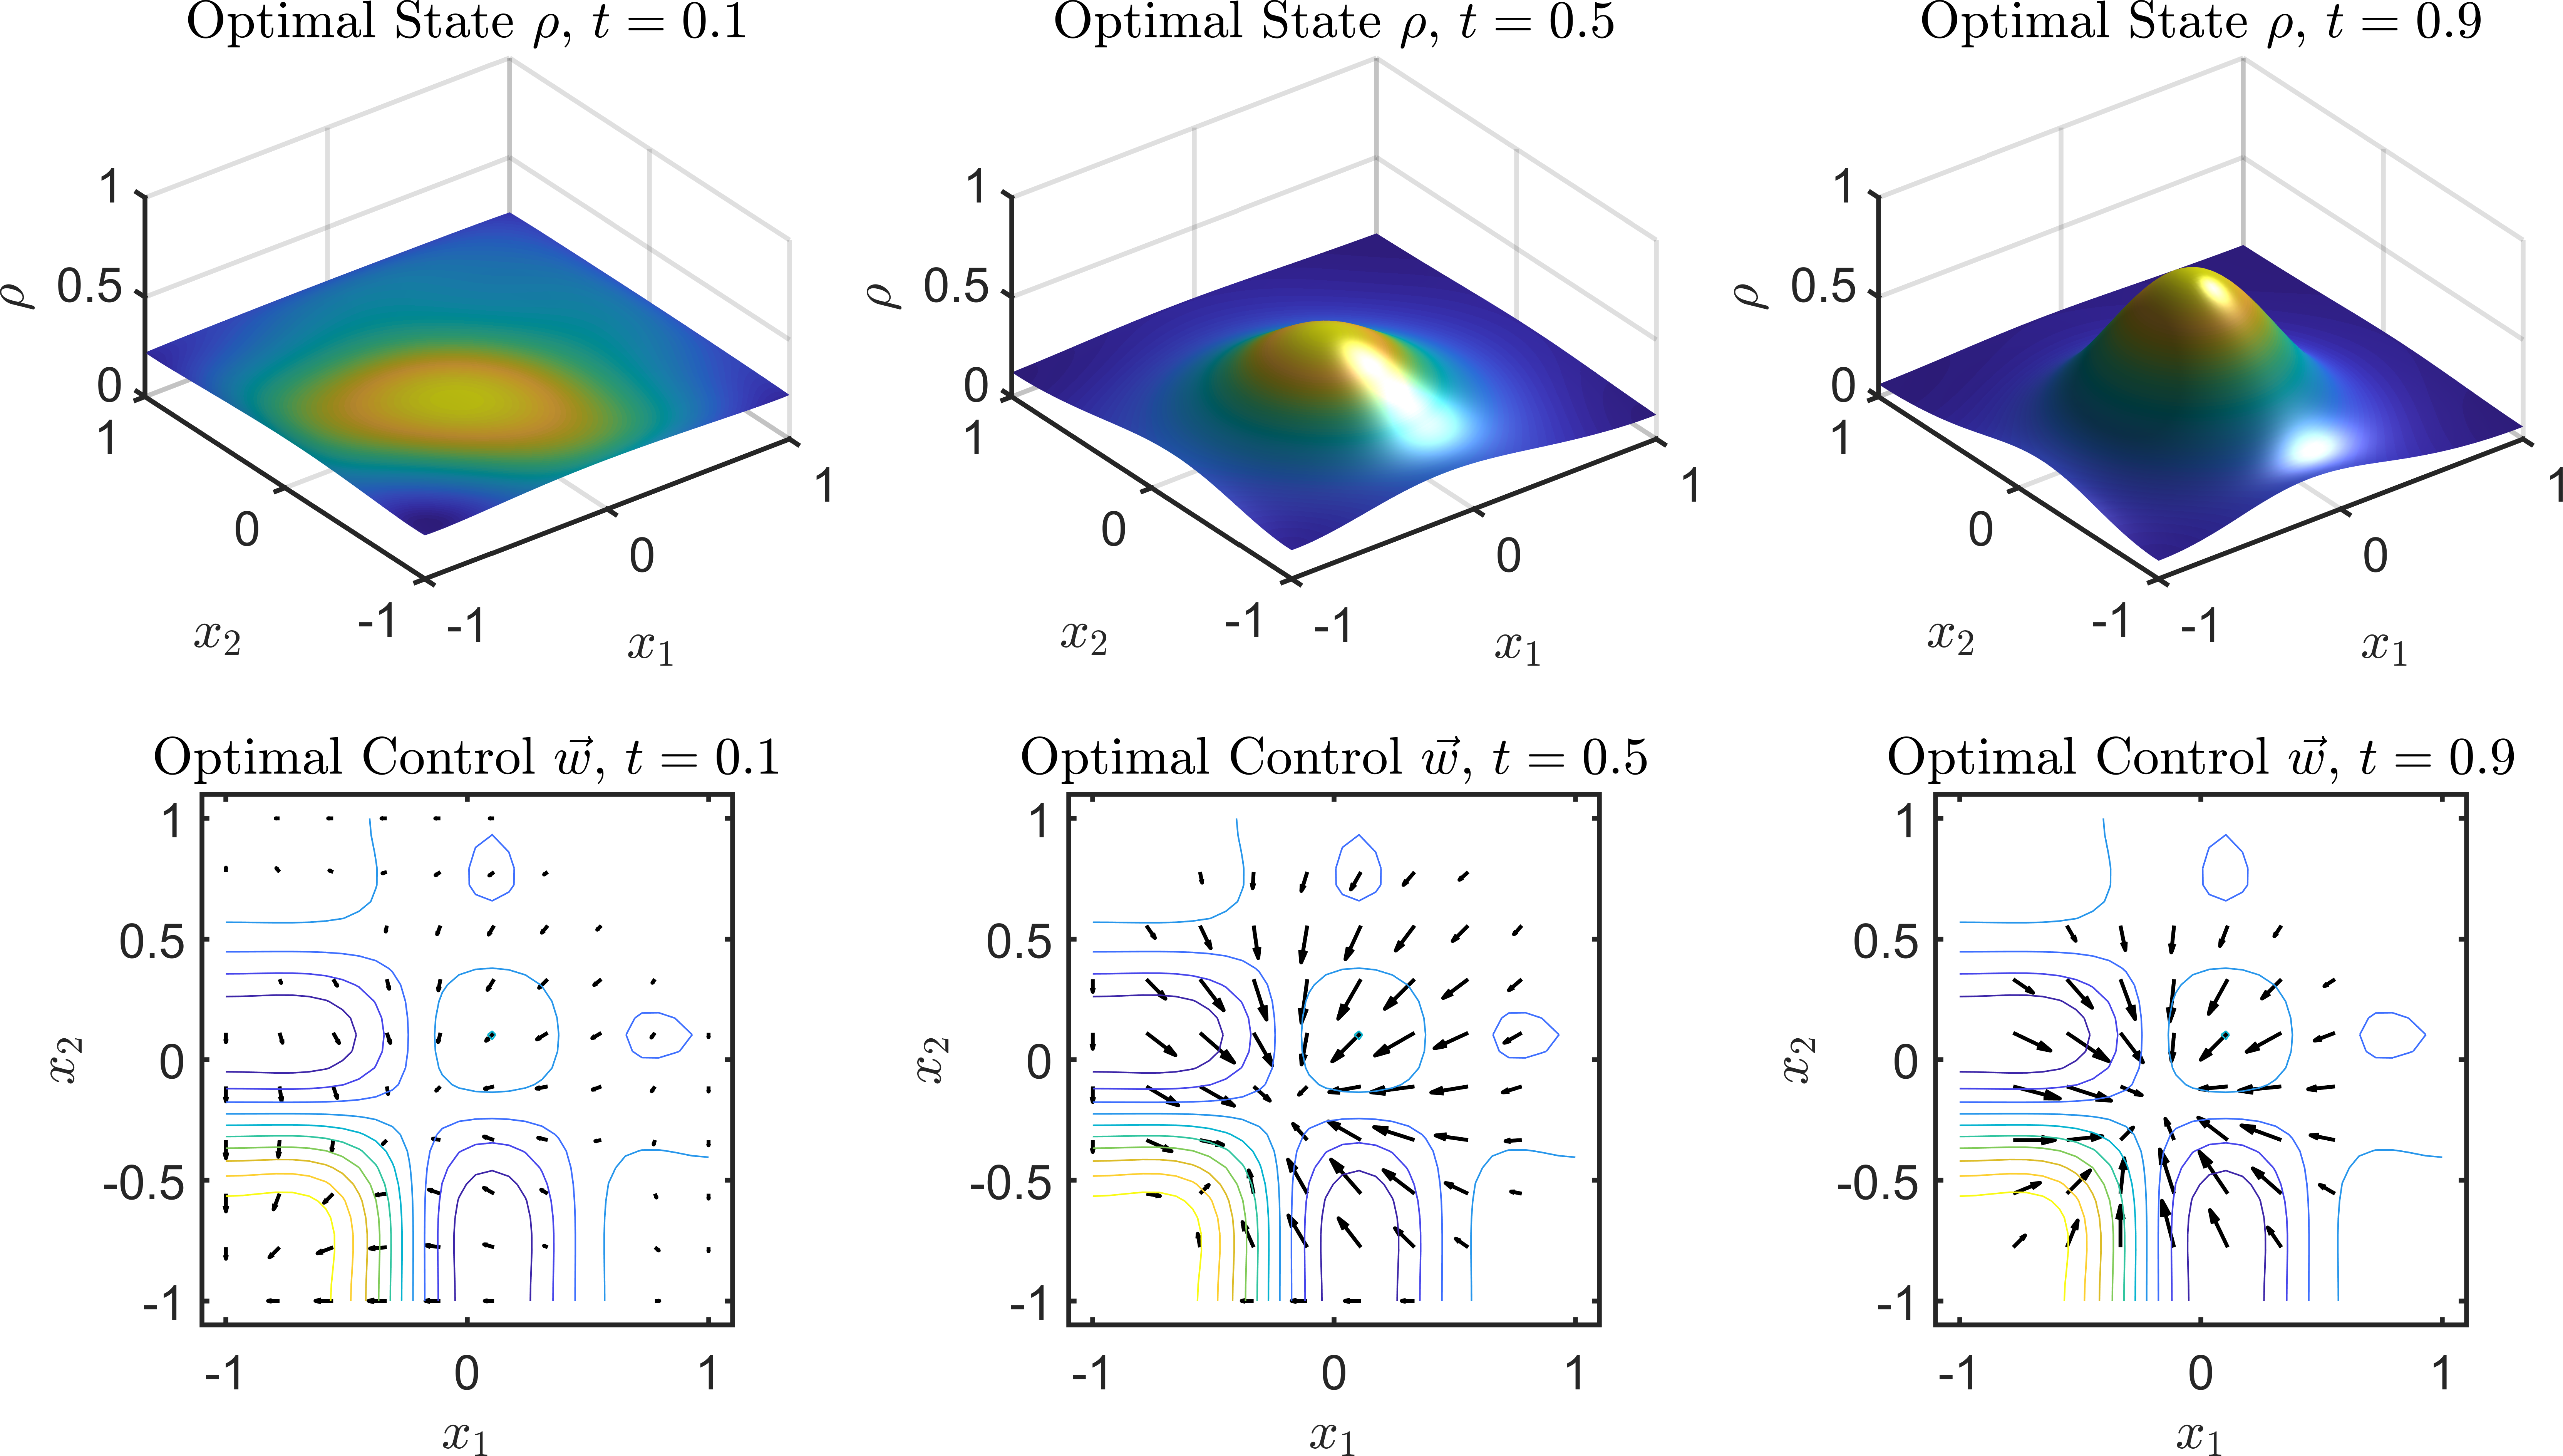
\includegraphics[scale=0.04]{Figure42D.png}
	\caption{2D Example 2, optimal state $\rho$ and optimal control $\vec{w}$, $\beta = 10^{-3}$, $\gamma = -1$.}
	\label{rhoOpt2dEx4}
\end{figure}







